%% The "\appendix" call has already been made in the declaration
%% of the "appendices" environment (see thesis.tex).

\chapter{Miscellaneous}
\section{Noise Filters}
\label{app:noise}

For Calo jets the following criteria were applied:

\begin{itemize}
  \item N90 hits $>$ 1, 
    \item  HBHE $>$ 0.01,
      \item fHPD $<$ 0.98,
\end{itemize}

For PF jets the following criteria were applied:
  
\begin{itemize}
  \item Neutral hadron fraction $<$ 0.99, 
    \item  Neutral EM fraction $<$ 0.99,
      \item Number of constituents $>$ 1,
        \item Charged hadron fraction $>$ 0,
          \item Charged multiplicity $>$ 0,
            \item Charged EM fraction $<$ 0.99.
\end{itemize}
  
The following noise filters are applied, to remove events with spurious, non-physical jets or missing transverse energy.

\begin{itemize}
  \item CSC tight beam halo filter,
    \item HBHE noise filter with isolated noise rejection,
      \item HCAL laser filter,
        \item ECAL dead cell trigger primitive (TP) filter,
          \item Tracking failure filter,
            \item Bad EE Supercrystal filter,
              \item ECAL Laser correction filter.
\end{itemize}

\section{Primary Vertices}

\label{app:primaryvertices}

The pileup per event is defined by the number of 'good' reconstructed primary vertices in the event, with each vertex satisfying the following requirements

\begin{itemize}
	\item $N_{dof} > 4$;
	\item vertex position along the bead direction of $\vert z_{vtx} \vert < 24$cm; 
	\item vertex position perpendicular to the beam of $\rho < 2$cm.

\end{itemize}


\chapter{L1 Jets}

\section{Leading Jet Energy Resolution}
\label{app:jetpuresolution}

\begin{figure}[htp]

    \centering
    \subfloat[]{  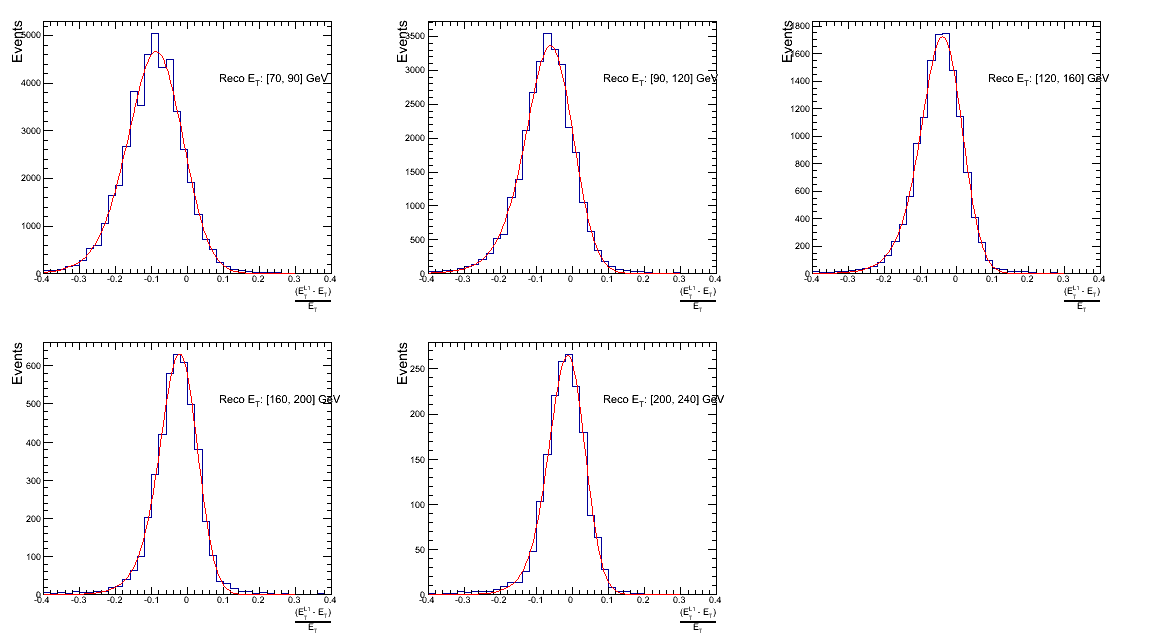
\includegraphics[width=0.95\textwidth]{plots/ptresolution_low.png}  }\,
\end{figure}

\begin{figure}
    \ContinuedFloat
    \centering
    \subfloat[]{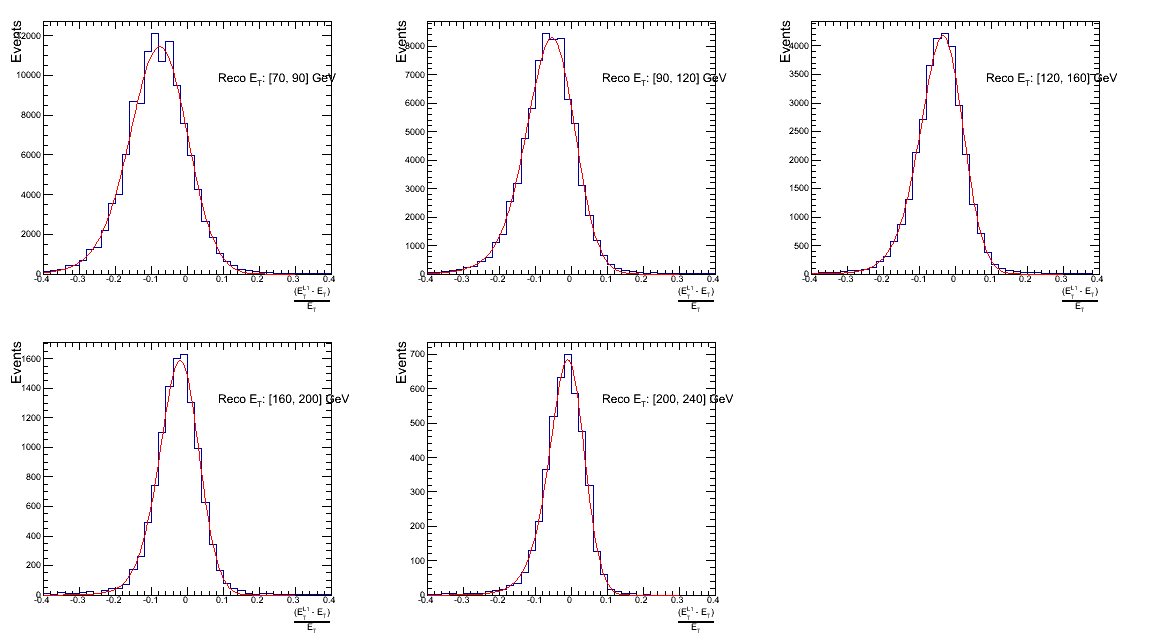
\includegraphics[width=0.95\textwidth]{plots/ptresolution_medium.png}}\,
    \subfloat[]{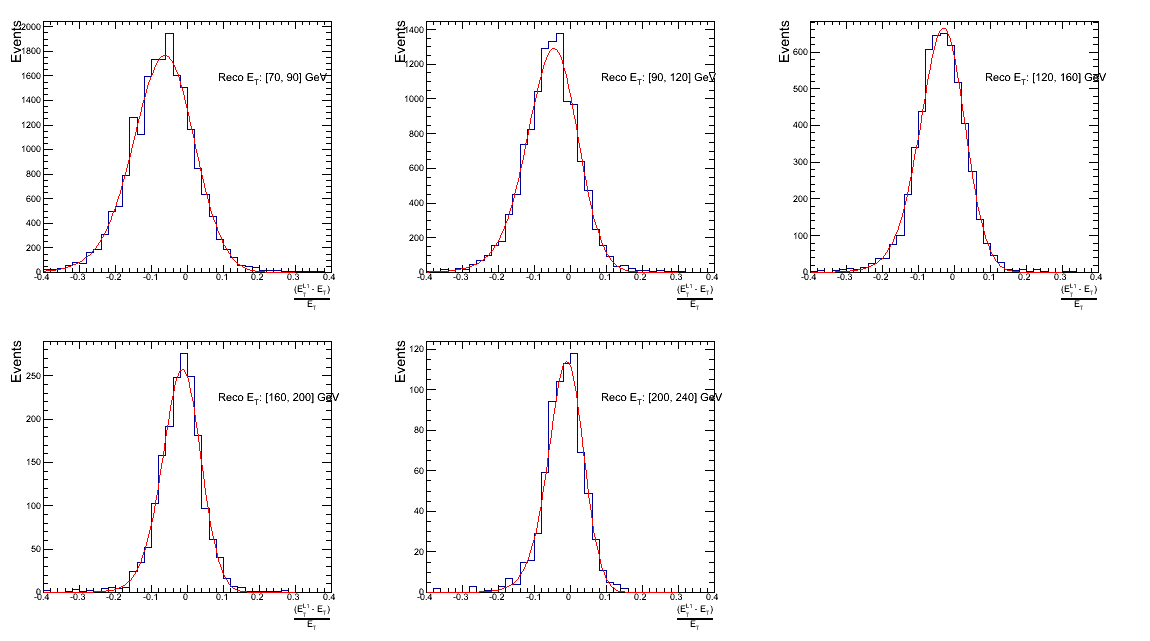
\includegraphics[width=0.95\textwidth]{plots/ptresolution_high.png}}\,

      \caption[ Resolution plots of the leading offline \Calo $\et$ measured as a function of  $\frac{(\text{L1 E}_{T} -  \text{Offline E}_{T})}{\text{Offline E}_{T}}$ for  low (a), medium (b) and high (c) pile-up conditions.] { Resolution plots of the leading offline jet \Calo $\et$ measured as a function of  $\frac{(\text{L1 E}_{T} -  \text{Offline E}_{T})}{\text{Offline E}_{T}}$ for  low (a), medium (b) and high (c) pile-up conditions. }
\end{figure}

\begin{figure}[htpb]

    \centering
    \subfloat[]{  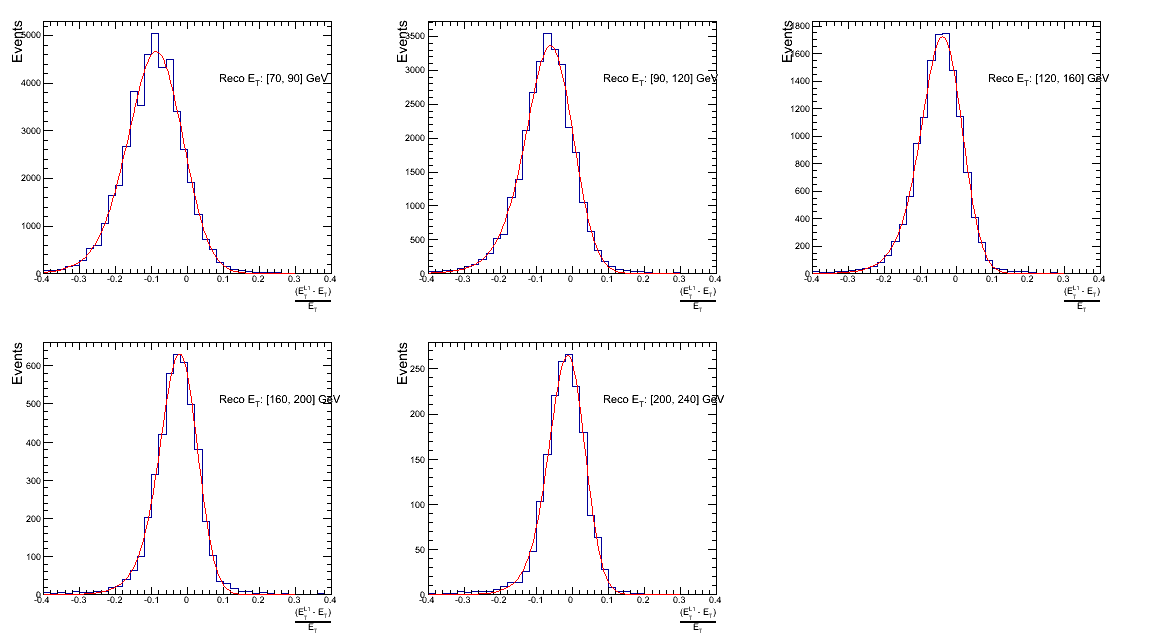
\includegraphics[width=0.95\textwidth]{plots/ptresolution_low.png}  }\,
    \subfloat[]{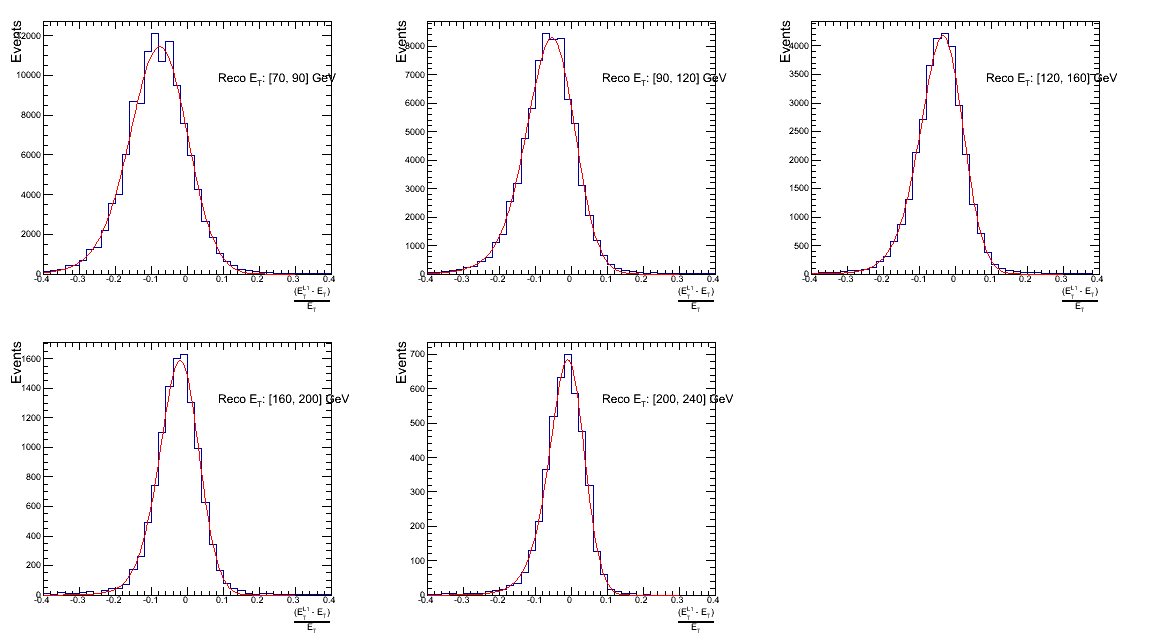
\includegraphics[width=0.95\textwidth]{plots/ptresolution_medium.png}}\,

\end{figure}

\begin{figure}
    \ContinuedFloat
    \centering
    \subfloat[]{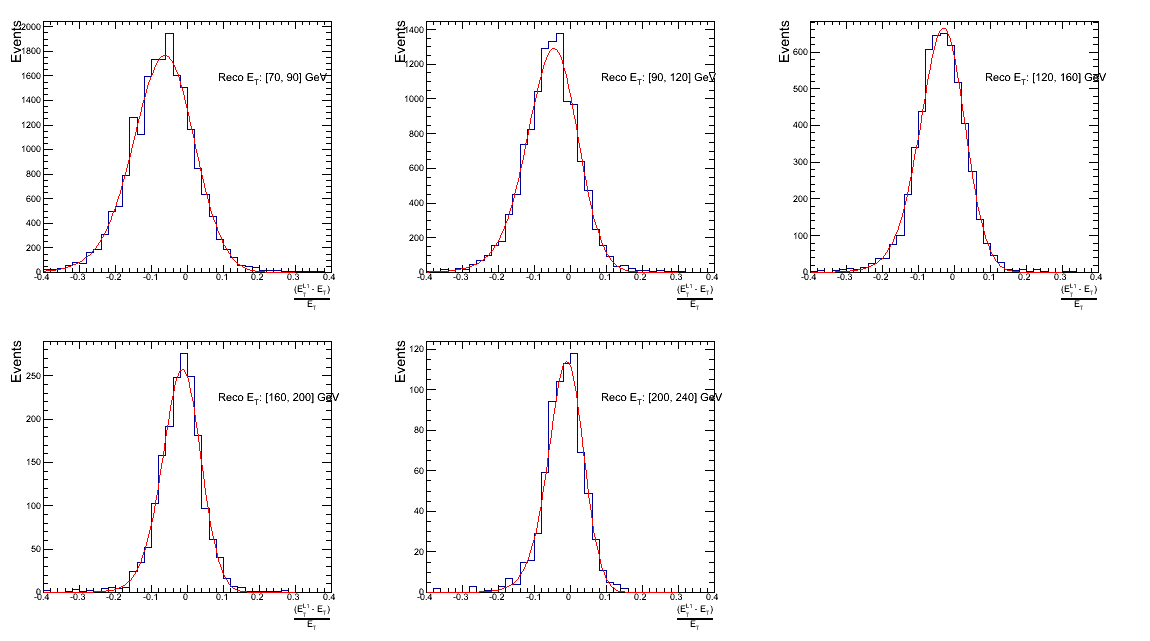
\includegraphics[width=0.95\textwidth]{plots/ptresolution_high.png}}\,

      \caption[ Resolution plots of the leading off-line PF $\et$ measured as a function of  $\frac{(\text{L1 E}_{T} -  \text{Offline E}_{T})}{\text{Offline E}_{T}}$ for  low (a), medium (b) and high (c) pile-up conditions.] { Resolution plots of the leading offline jet \PF $\et$ measured as a function of  $\frac{(\text{L1 E}_{T} -  \text{Offline E}_{T})}{\text{Offline E}_{T}}$ for  low (a), medium (b) and high (c) pile-up conditions. }
  
\end{figure}


\newpage
\section{Resolution for Energy Sum Quantities}
\label{app:jetenergysums}

The following plots show the resolution parameters for the four energy sum quantities as a function of the quantity (q) itself. In this case, The mean and RMS of the individual $\frac{(\text{L1 q} -  \text{Offline q})}{\text{Offline q}}$ distributions, in bins of the quantity q is displayed. 

\begin{figure}[h!]
  \vspace{20pt}
        \centering
        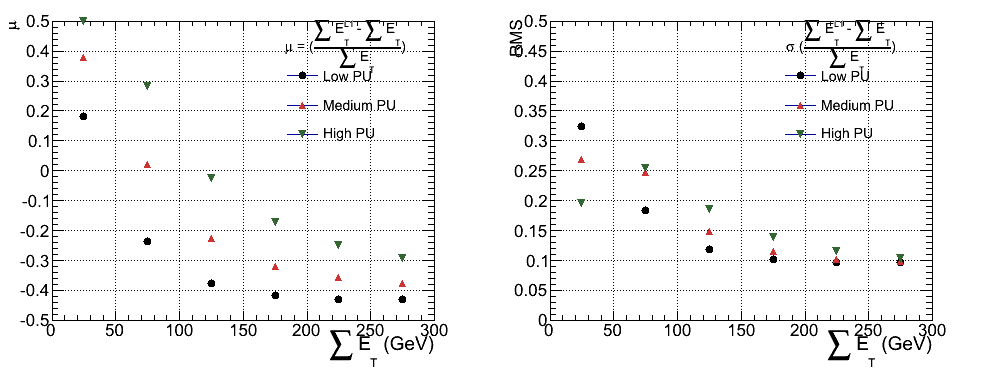
\includegraphics[width=1.0\textwidth]{plots/res_CaloSumET_summary.png}
        \caption{$\sum$ $\et$~resolution parameters in bins of Calo $\sum E_{T}$  measured for the defined low, medium and high pile up conditions. The plots show the mean $\mu$ (left), resolution $\sigma$ (RMS) of the $\frac{\Delta q}{q}$ distributions.}
        \label{fig:caloetresultspu}
\end{figure}
\begin{figure}[h!]
  \vspace{20pt}
  \centering
        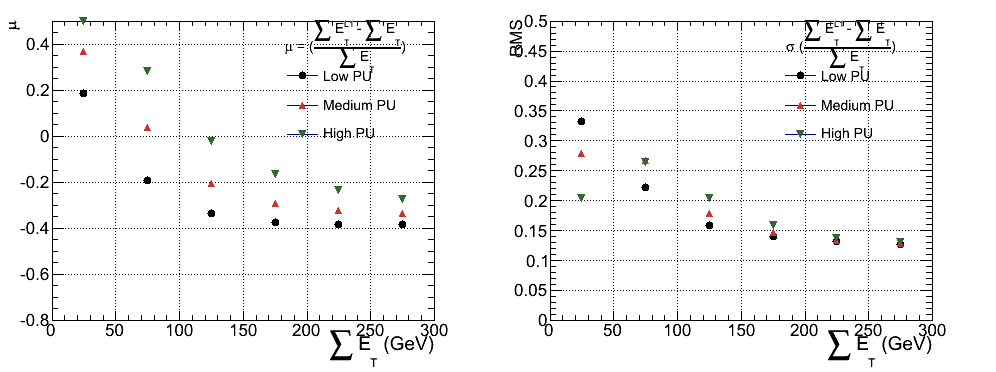
\includegraphics[width=1.0\textwidth]{plots/res_pfSumET_summary.png}
        \caption{$\sum$ $\et$~resolution parameters in bins of PF $\sum E_{T}$  measured for the defined low, medium and high pile up conditions. The plots show the mean $\mu$ (left), resolution $\sigma$ (RMS) of the $\frac{\Delta q}{q}$ distributions.}
        \label{fig:pfetresultspu}
\end{figure}

\begin{figure}[h!]
  \vspace{20pt}
        \centering
        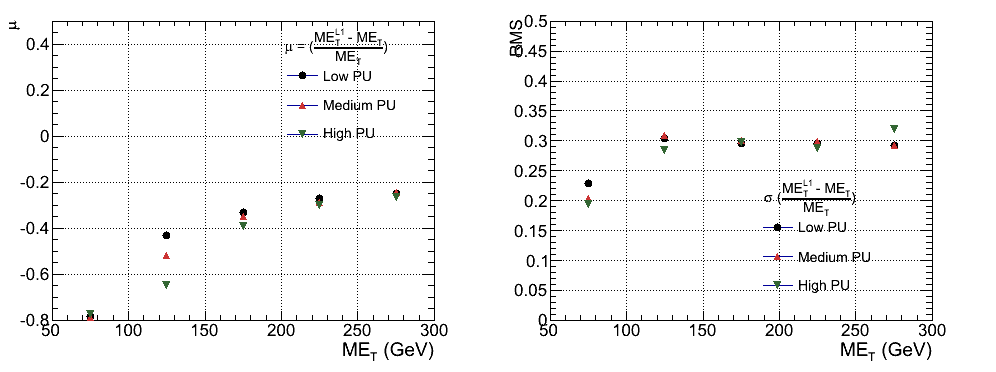
\includegraphics[width=1.0\textwidth]{plots/res_CaloMET_summary.png}
        \caption{$\met$~resolution parameters in bins of Calo $\met$~ measured for the defined low, medium and high pile up conditions. The plots show the mean $\mu$ (left), resolution $\sigma$ (RMS) of the $\frac{\Delta q}{q}$  distributions.}
        \label{fig:calometresultspu}
\end{figure}
\begin{figure}[h!]
  \vspace{20pt}
        \centering
        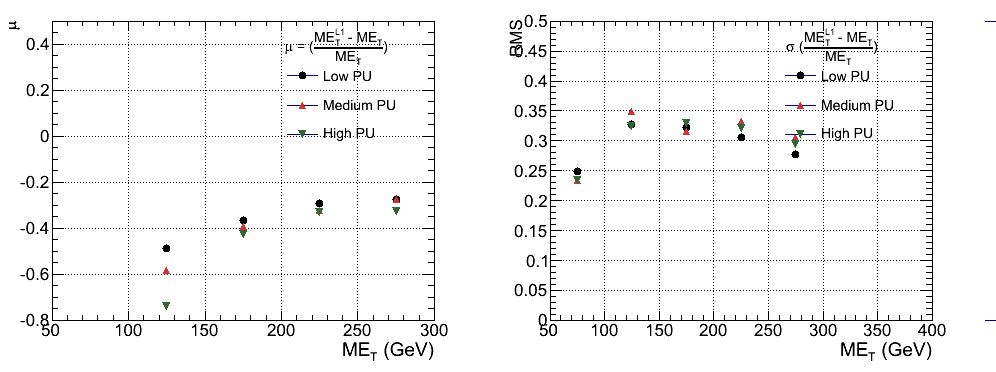
\includegraphics[width=1.0\textwidth]{plots/res_pfMET_summary.png}
        \caption{$\met$~resolution parameters in bins of PF $\met$~ measured for the defined low, medium and high pile up conditions. The plots show the mean $\mu$ (left), resolution $\sigma$ (RMS) of the $\frac{\Delta q}{q}$  distributions.}
        \label{fig:pfmetresultspu}
\end{figure}


\begin{figure}[h!]
  \vspace{20pt}
        \centering
        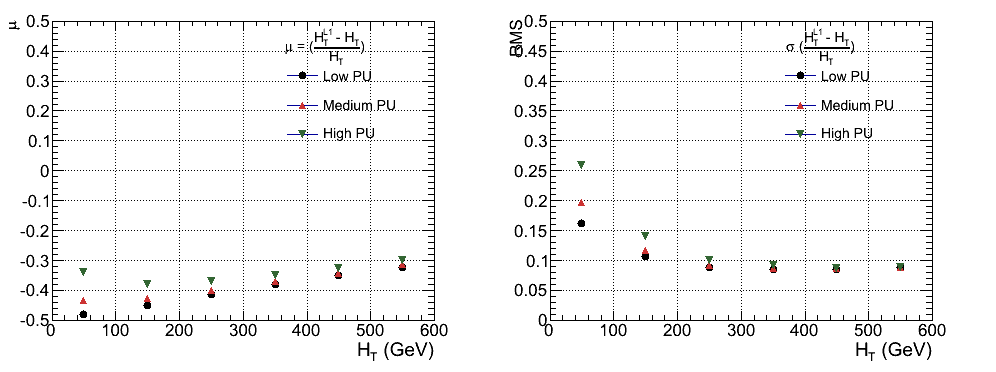
\includegraphics[width=1.0\textwidth]{plots/res_CaloHT_summary.png}
        \caption{$\theht$~resolution parameters in bins of Calo $\theht$~measured for the defined low, medium and high pile up conditions. The plots show the mean $\mu$ (left), resolution $\sigma$ (RMS) of the $\frac{\Delta q}{q}$ distributions.}
        \label{fig:calohtresultspu}
\end{figure}
\begin{figure}[h!]
  \vspace{20pt}
        \centering
        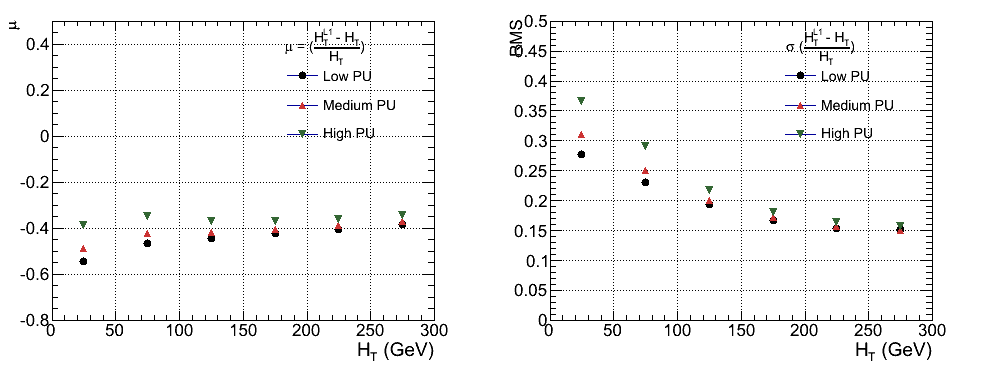
\includegraphics[width=1.0\textwidth]{plots/res_pfHT_summary.png}
        \caption{$\theht$~resolution parameters in bins of PF $\theht$~measured for the defined low, medium and high pile up conditions. The plots show the mean $\mu$ (left), resolution $\sigma$ (RMS) of the $\frac{\Delta q}{q}$ distributions.}
        \label{fig:pfhtresultspu}
\end{figure}

\begin{figure}[h!]
  \vspace{20pt}
        \centering
        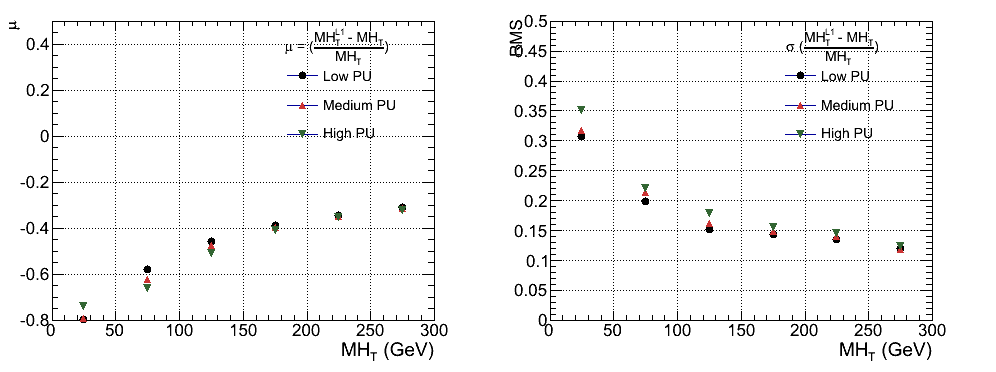
\includegraphics[width=1.0\textwidth]{plots/res_CaloMHT_summary.png}
        \caption{$\mht$~resolution parameters in bins of $\mht$~measured for the defined low, medium and high pile up conditions. The plots show the mean $\mu$ (left), resolution $\sigma$ (RMS) of the $\frac{\Delta q}{q}$ distributions.}
        \label{fig:calomhtresultspu}
\end{figure}
\begin{figure}[h!]
  \vspace{20pt}
        \centering
        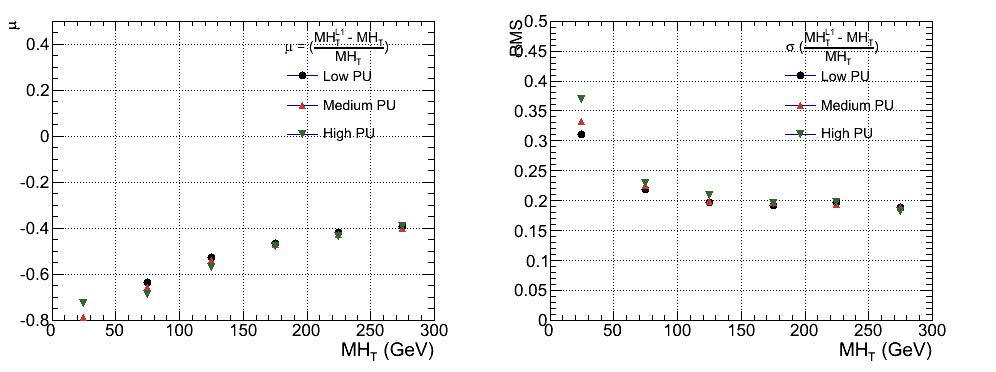
\includegraphics[width=1.0\textwidth]{plots/res_pfMHT_summary.png}
        \caption{$\mht$~resolution parameters in bins of PF $\mht$~measured for the defined low, medium and high pile up conditions. The plots show the mean $\mu$ (left), resolution $\sigma$ (RMS) of the $\frac{\Delta q}{q}$ distributions.}
        \label{fig:pfmhtresultspu}
\end{figure}






